\documentclass[a4paper]{article}

\usepackage[pages=all, color=black, position={current page.south}, placement=bottom, scale=1, opacity=1, vshift=5mm]{background}
%\SetBgContents{
%	\tt This work is shared under a \href{https://creativecommons.org/licenses/by-sa/4.0/}{CC BY-SA 4.0 license} unless otherwise noted
%}      % copyright

\usepackage[margin=1in]{geometry} % full-width

% AMS Packages
\usepackage{amsmath}
\usepackage{amsthm}
\usepackage{amssymb}

% Unicode
\usepackage[utf8]{inputenc}
\usepackage{hyperref}
\hypersetup{
	unicode,
%	colorlinks,
%	breaklinks,
%	urlcolor=cyan, 
%	linkcolor=blue, 
	pdfauthor={Author One, Author Two, Author Three},
	pdftitle={A simple article template},
	pdfsubject={A simple article template},
	pdfkeywords={article, template, simple},
	pdfproducer={LaTeX},
	pdfcreator={pdflatex}
}

% Natbib
\usepackage[sort&compress,numbers,square]{natbib}
\bibliographystyle{mplainnat}

% Theorem, Lemma, etc
\theoremstyle{plain}
\newtheorem{theorem}{Theorem}
\newtheorem{corollary}[theorem]{Corollary}
\newtheorem{lemma}[theorem]{Lemma}
\newtheorem{claim}{Claim}[theorem]
\newtheorem{axiom}[theorem]{Axiom}
\newtheorem{conjecture}[theorem]{Conjecture}
\newtheorem{fact}[theorem]{Fact}
\newtheorem{hypothesis}[theorem]{Hypothesis}
\newtheorem{assumption}[theorem]{Assumption}
\newtheorem{proposition}[theorem]{Proposition}
\newtheorem{criterion}[theorem]{Criterion}
\theoremstyle{definition}
\newtheorem{definition}[theorem]{Definition}
\newtheorem{example}[theorem]{Example}
\newtheorem{remark}[theorem]{Remark}
\newtheorem{problem}[theorem]{Problem}
\newtheorem{principle}[theorem]{Principle}

\usepackage{graphicx, color}
\graphicspath{{fig/}}

%\usepackage[linesnumbered,ruled,vlined,commentsnumbered]{algorithm2e} % use algorithm2e for typesetting algorithms
\usepackage{algorithm, algpseudocode} % use algorithm and algorithmicx for typesetting algorithms
\usepackage{mathrsfs} % for \mathscr command

% Author info
\title{Andy's science scratch pad}
\author{J. Andrew Fingerhut (\texttt{andy.fingerhut@gmail.com})}

\date{
        May 31, 2025
%	\today
}

\newcommand{\ihat}{\textbf{i}}
\newcommand{\jhat}{\textbf{j}}
\newcommand{\khat}{\textbf{k}}
\newcommand{\rhat}{\hat{\textbf{r}}}
\newcommand{\vect}[1]{\textbf{#1}}

\begin{document}
\maketitle

%\begin{abstract}
%  todo: abstract here
%\end{abstract}

\tableofcontents

\section{Introduction}
\label{sec:intro}

This document is a place to write up little bits on science.

Some notation:

$\ihat$ is the unit vector from left to right.
$\jhat$ is the unit vector upwards.
$\khat$ is the unit vector pointed out of the page toward the reader.

$\gamma = 1/\sqrt{1-v^2/c^2}$ is the Lorentz factor.


\section{Electromagnetic force between two point charges at rest relative to each other}
\label{sec:twocharges}

Scenario 1: There are two point charges $a$ and $b$ both with charge
$q$ at rest relative to each other at a distance $r$ apart (see
Figure~\ref{fig:two-charges-at-rest}).  They are at rest relative
to us.  In this case they both experience a force directly away from
the other due to electric repulsion.  There is no magnetic force, as
both charges are at rest so there are no magnetic fields.

\begin{figure}[ht]
	\centering
	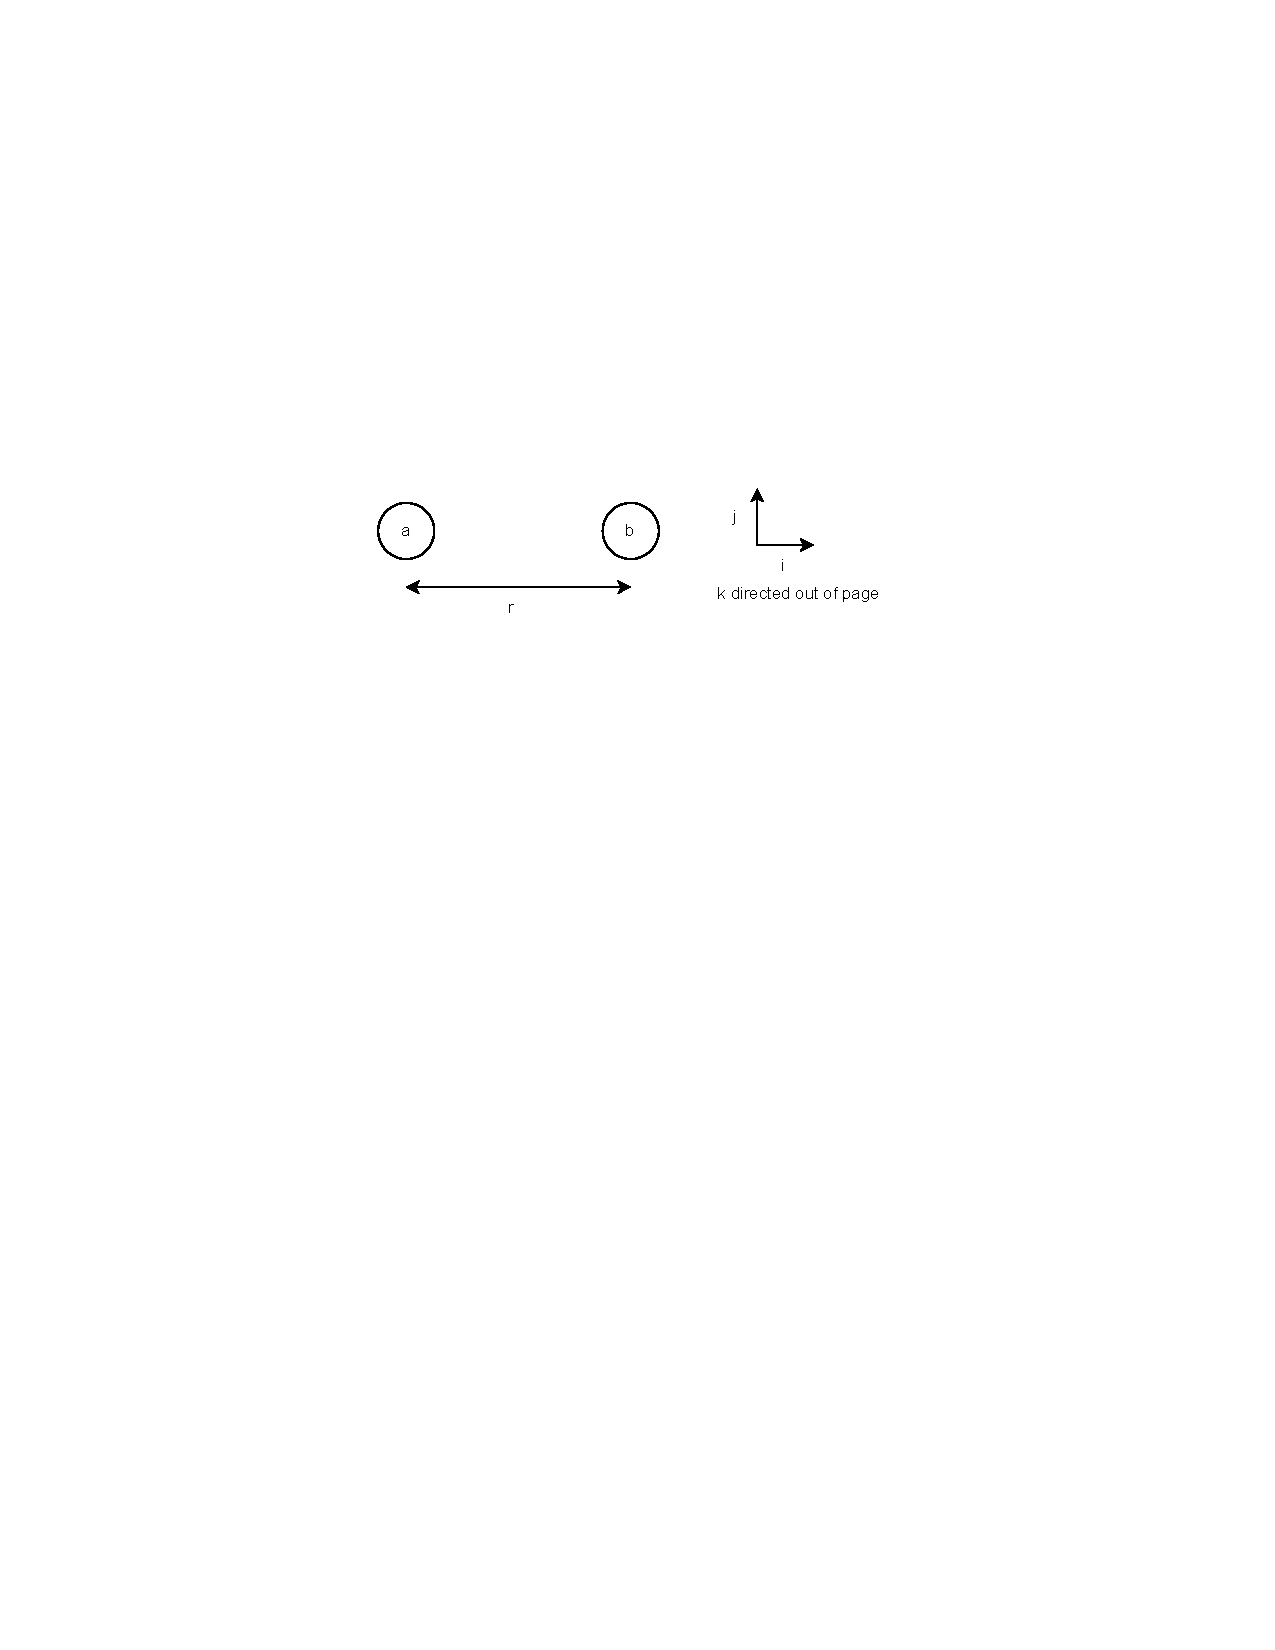
\includegraphics[width=0.6\textwidth]{two-charges-at-rest-cropped.pdf}
	\caption{Two point charges at rest}
	\label{fig:two-charges-at-rest}
\end{figure}


Scenario 2: The same as scenario 1, but both charges are moving with
constant velocity $v$ in the upwards direction (see
Figure~\ref{fig:two-charges-moving}).  Since they are moving they
create magnetic fields.

\begin{figure}[ht]
	\centering
	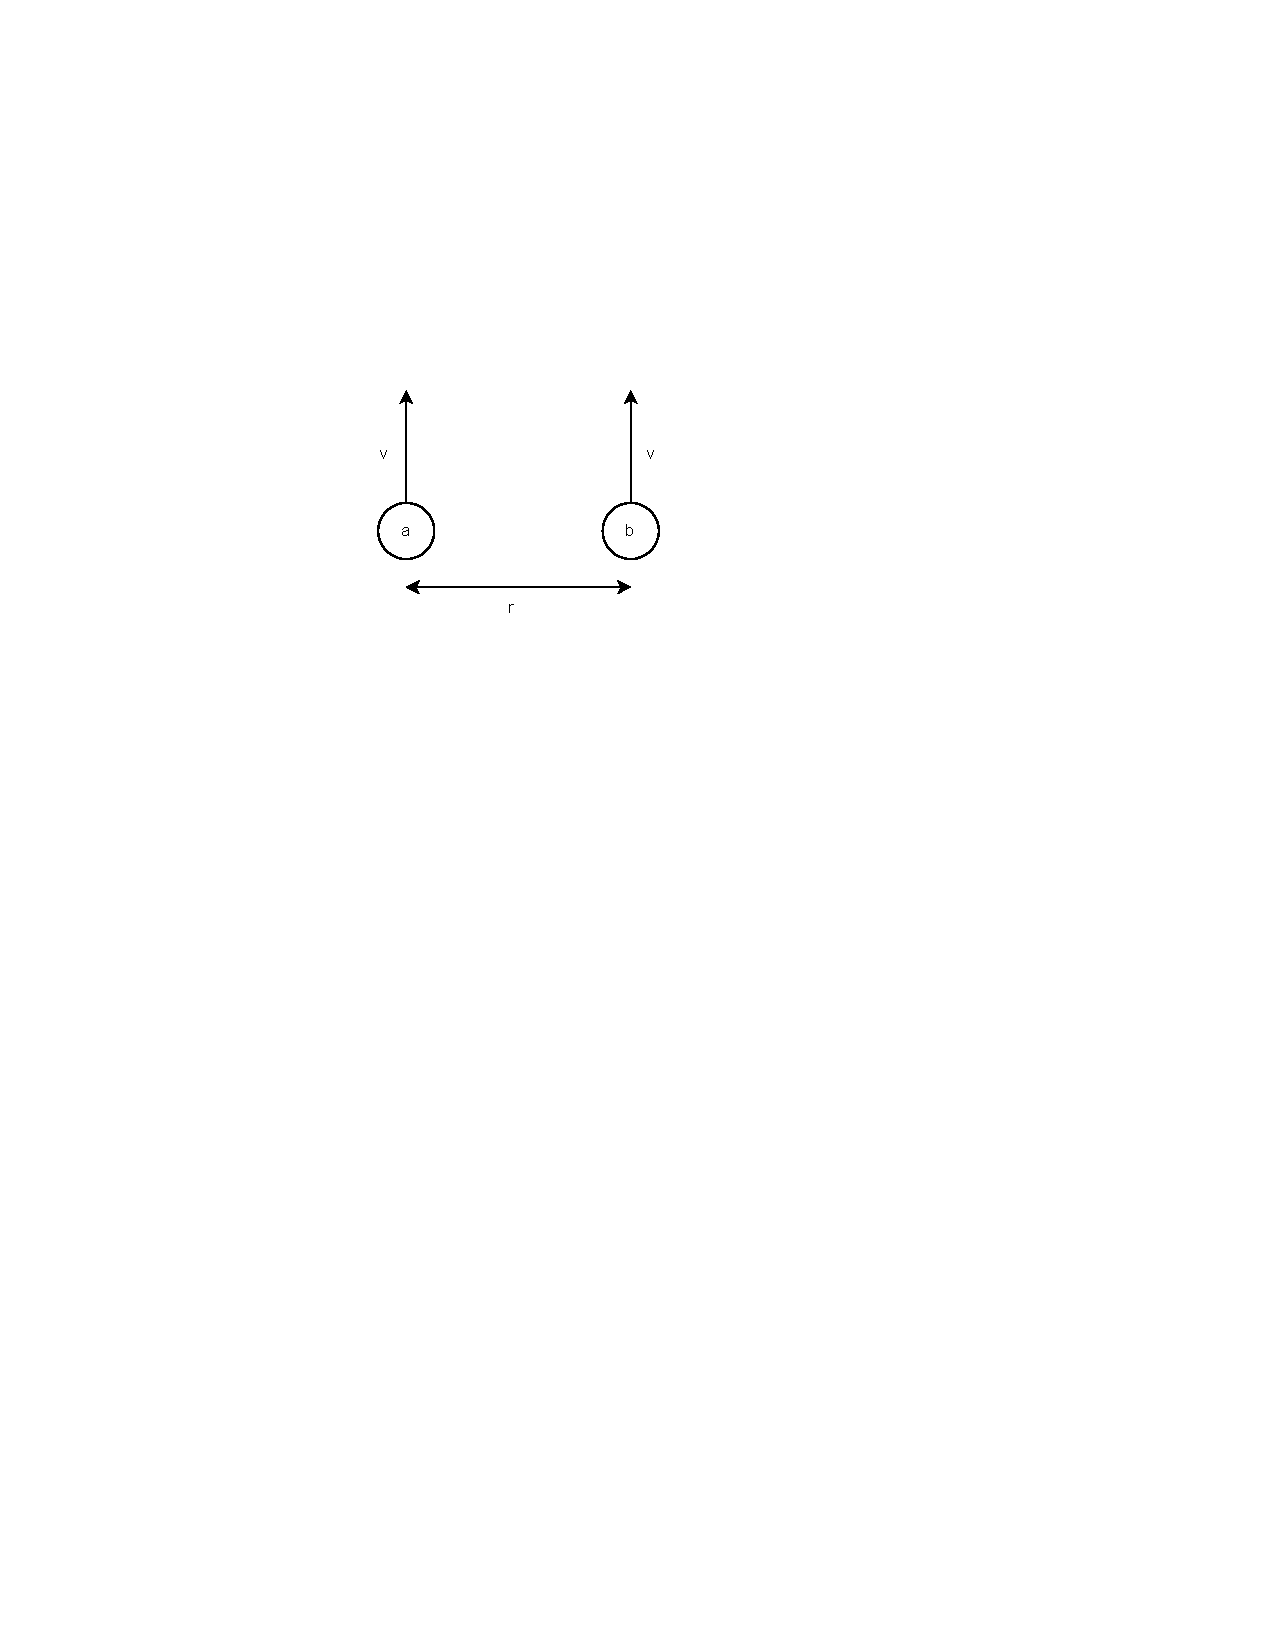
\includegraphics[width=0.4\textwidth]{two-charges-moving-cropped.pdf}
	\caption{Two point charges moving at same constant velocity}
	\label{fig:two-charges-moving}
\end{figure}

Questions:
\begin{itemize}
  \item What is the net force on charge $b$ in each scenario?
  \item Is it the same in both scenarios, or different?
  \item Why?
\end{itemize}


\subsection{Scenario 1: Both charges at rest}

As mentioned before, there is no current or motion of any charges in
this scenario, so no magnetic fields.  The electric repulsion force on
charge $b$ is easily calculated from Coulomb's Law~\cite{CoulombsLaw}.
Charge $b$ is to the right of charge $a$, so the direction of the force is
$\ihat$, away from charge $a$.

\begin{equation}
\vect{E}_1 = \frac{1}{4 \pi \epsilon_0} \frac{q}{r^2} \ihat \label{eq:E1}
\end{equation}

\begin{equation}
\vect{B}_1 = 0
\end{equation}

\begin{equation}
\vect{F}_1 = q(\vect{E}_1 + \vect{v} \times \vect{B}_1)
           = q \vect{E}_1   \label{eq:F1}
\end{equation}


\subsection{Scenario 2: Both charges with equal and constant velocity upwards}

\subsubsection{Scenario 2 calculated by electromagnetic field equations from Griffiths}

The Wikipedia page on the Biot-Savart
Law~\cite{EMFieldFromPointCharge} has a subsection titled ``Point
charge at constant velocity'' that says:

\begin{quote}
the Biot–Savart law applies only to steady currents and a point charge
moving in space does not constitute a steady current
\end{quote}

I will thus use the equations in that section to calculate the
electric and magnetic fields here.  The relevant parts of the
Wikipedia page are copied below.

\begin{quote}
In the case of a point charged particle $q$ moving at a constant
veclocity $\vect{v}$, Maxwell's equations give the following
expression for the electric field and magnetic field:
\end{quote}
\begin{align}
\vect{E} & = \frac{q}{4 \pi \epsilon_0} \frac{1-\beta^2}{(1-\beta^2 \sin^2 \theta)^{3/2}} \frac{{\rhat}'}{|r'|^2} \label{eq:EforPtChg} \\
\vect{B} & = \frac{1}{c^2} \vect{v} \times \vect{E} \label{eq:BforPtChg}
\end{align}
where:
\begin{itemize}
    \item ${\rhat}'$ is the unit vector pointing from the current
      (non-retarded) position of the particle to the point at which
      the field is being measured,
    \item $\beta = v/c$ is the speed in units of $c$, and
    \item $\theta$ is the angle between $\vect{v}$ and ${\rhat}'$.
\end{itemize}

The equations above appear to be identical to equations (10.75) and
(10.76) in Griffiths~\cite{Griffiths1998}.  Griffiths comments on the formula for the electric field:

\begin{quote}
Notice that $\vect{E}$ points along the line from the {\em present}
position of the particle.  This is an extraordinary coincidence, since
the ``message'' came from the retarded position.  Because of the
$\sin^2 \theta$ in the denominator, the field of a fast-moving charge
is flattened out like a pancake in the direction perpendicular to the
motion (Fig. 10.10).  In the forward and backward directions
$\vect{E}$ is reduced by a factor $(1 - v^2/c^2)$ relative to the
field of a charge at rest; in the perpendicular direction it is
{\em enhanced} by a factor $1 / \sqrt{ 1 - v^2/c^2}$.
\end{quote}

Calculation: To get the force on charge $b$, we first calculate the
$\vect{E}$ and $\vect{B}$ fields at the position of charge $b$.

Charge $b$ is directly to the right of charge $a$, so ${\rhat}' = \ihat$
and $\theta = 90^{\circ}$.

\begin{align}
\vect{E}_2
  & = \frac{q}{4 \pi \epsilon_0} \frac{1-\beta^2}{(1-\beta^2 \sin^2 \theta)^{3/2}} \frac{{\rhat}'}{|r'|^2} & & \text{${\rhat}' = \ihat$, $|r'| = r$, $\theta=90^{\circ}$, simplify fraction} \nonumber \\
  & = \frac{q}{4 \pi \epsilon_0} \frac{1}{(1-\beta^2)^{1/2}} \frac{\ihat}{r^2} & & \text{part of this is $\gamma$, by~\eqref{eq:E1} the rest is $\vect{E}_1$} \nonumber \\
  & = \gamma \vect{E}_1 \label{eq:E2value}
\end{align}

Note that $\vect{E}_2$ being $\gamma$ times larger than $\vect{E}_1$
is consistent with the comment from Griffiths above: ``in the
perpendicular direction it ($\vect{E}$) is {\em enhanced} by a factor
$1 / \sqrt{ 1 - v^2/c^2}$''.

\begin{align*}
\vect{F}_2
  & = q (\vect{E}_2 + \vect{v} \times \vect{B}_2)   & & \text{replace $\vect{B}_2$ with \eqref{eq:BforPtChg}} \\
  & = q (\vect{E}_2 + \vect{v} \times (\frac{1}{c^2} \vect{v} \times \vect{E}_2))  & & \vect{v} \times \vect{E}_2 = - v E_2 \khat \\
  & = q (\vect{E}_2 - \frac{v E_2}{c^2} \vect{v} \times \khat)  & & \vect{v} \times \khat = v \ihat \\
  & = q (\vect{E}_2 - \frac{v^2 E_2}{c^2} \ihat) \\
  & = q (1 - \frac{v^2}{c^2}) \vect{E}_2 \\
  & = \frac{q \vect{E}_2}{\gamma^2} & & \text{by~\eqref{eq:E2value} \ } \vect{E}_2 = \gamma \vect{E}_1 \\
  & = \frac{q \vect{E}_1}{\gamma} & & \text{by~\eqref{eq:F1} \ } \vect{F}_1 = q \vect{E}_1 \\
  & = \frac{\vect{F}_1}{\gamma}
\end{align*}

Thus $\vect{F}_2$ differs from $\vect{F}_1$ by a factor of $\gamma$.

TODO: Why?

I do not know how to check the answer below, but it appears that three
of the answers to an on-line question similar to
mine~\cite{PhysicsSEIsLorentzForceFrameIndependent} say that the
Lorentz force formula $\vect{F} = q(\vect{E} + \vect{v} \times
\vect{B})$ is {\em not} invariant in all inertial frames, but perhaps
a slightly modified version of that formula is invariant between
different inertial frames.  I quote one such answer below:

\begin{quote}
Just for completeness if permitted: Following Section 3.1 from the
book ``Gravitation'' of Misner, Thorne, and Wheeler the truly (at all
speeds) frame independent force is $\frac{dP}{d \tau} = \gamma (E + v
\times B)$ (in fact this is only the spacial component of the four
force).  $\tau$ is proper time and $\gamma$ the well-known Lorentz
Factor. -- Kurt G. Aug 28, 2021
\end{quote}


\subsubsection{Scenario 2 calculated by Heaviside-Feynman formula}

The Wikipedia page on Jefimenko's Equations~\cite{JefimenkosEquations}
has a subsection titled ``Heaviside-Feynman formula'' that gives
equations for the electric and magnetic field at a point due to a
single moving point charge.

\begin{align}
\vect{E} & = \frac{-q}{4 \pi \epsilon_0}
             \left[
               \frac{\vect{e}_{r'}}{r'^2}
               + \frac{r'}{c} \frac{d}{dt} \left( \frac{\vect{e}_{r'}}{r'^2} \right)
               + \frac{1}{c^2} \frac{d^2}{dt^2} \vect{e}_{r'}
             \right]
             \label{eq:HF-EforPtChg} \\
\vect{B} & = - \vect{e}_{r'} \times \frac{\vect{E}}{c}
             \label{eq:HF-BforPtChg}
\end{align}

Here $\vect{e}_{r'}$ is a unit vector pointing from the observer to
the charge and $r'$ is the distance between observer and charge.
Since the electromagnetic field propagates at the speed of light, both
of these quantities are evaluated at the retarted time $t - r'/c$.

I believe ``observer'' above means ``the position for which we are
calculating $E$ and $B$ fields''.

Assume here that the point charges are kept at distance $r$ apart from
each other, always horizontally, e.g. because they are connected by a
stiff insulating rod.  This simplifies our job of calculating $E$,
because then $\vect{e}_{r'}$ and $r'$ are unchanging over time, and
their derivates are thus 0.

We want to calculate $r'$ as the vector from the position of charge
$b$ to the position where charge $a$ was when it emitted an electric
field propagated at speed $c$ to $b$.  See
Figure~\ref{fig:retarded-position}.

\begin{figure}[ht]
	\centering
	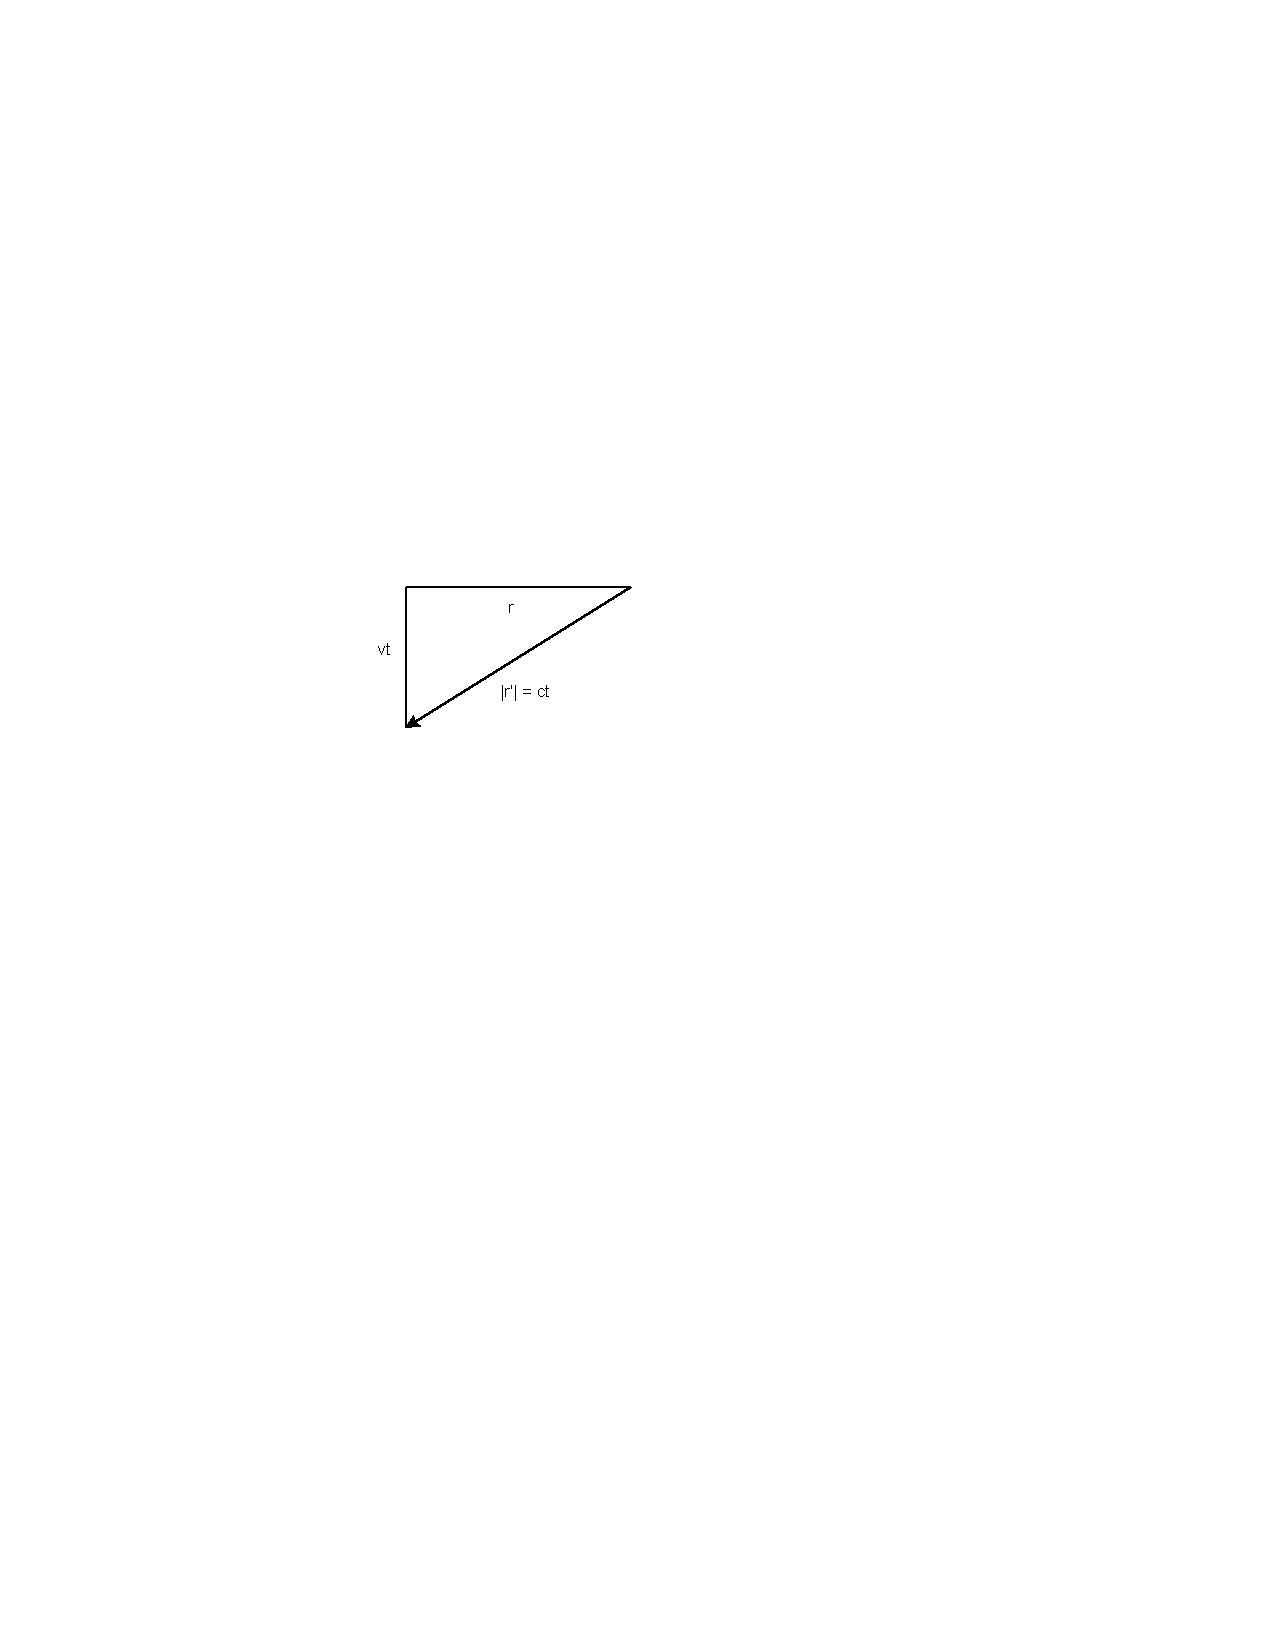
\includegraphics[width=0.5\textwidth]{retarded-position-cropped.pdf}
	\caption{The retarded position of charge $a$ from charge $b$}
	\label{fig:retarded-position}
\end{figure}

Solve for $t$ using Pythagorean theorem since $r$ and $v$ are known
constants:
\begin{align*}
r^2 + (vt)^2 & = (ct)^2 \\
t^2 (c^2 - v^2) & = r^2 \\
t^2 & = \frac{r^2}{c^2 - v^2} \\
t & = \frac{r}{\sqrt{c^2-v^2}} \\
  & = \frac{r}{c \sqrt{1 - v^2/c^2}} \\
  & = \gamma r / c
\end{align*}

This gives us $r' = ct = \gamma r$, and $\vect{e}_{r'}$ is:

\begin{align*}
\vect{e}_{r'} & = \frac{-r \ihat - (\gamma r v / c) \jhat}{\gamma r} \\
  & = - \frac{1}{\gamma} \ihat - \frac{v}{c} \jhat
\end{align*}

Plugging in this value for $\vect{e}_{r'}$ into
Equation~\eqref{eq:HF-EforPtChg} gives:

\begin{align*}
\vect{E}_3 & = \frac{q}{4 \pi \epsilon_0}
             \left[
               \frac{\frac{1}{\gamma} \ihat + \frac{v}{c} \jhat}{\gamma^2 r^2}
             \right]
\end{align*}

Note that $\vect{E}_3$ is parallel to $\vect{e}_{r'}$, thus
$\vect{B}_3$ from Equation~\eqref{eq:HF-BforPtChg} is 0.

This gives the force on charge $b$ as:
\begin{align*}
\vect{F}_3
  & = q (\vect{E}_3 + \vect{v} \times \vect{B}_3) \\
  & = q \vect{E}_3
\end{align*}
The direction of $\vect{F}_3$ is different than $\vect{F}_1$ and $\vect{F}_2$.
Below is the relative magnitude of $\vect{E}_3$ to $\vect{E}_1$:
\begin{align*}
E_3 & = \frac{1}{\gamma^2} E_1 \\
F_3 & = \frac{1}{\gamma^2} F_1
\end{align*}

TODO: It seems {\em very} odd to me that $\vect{B}_3 = 0$.

After Feynman explains what the retarded direction and distance
$\vect{r'}$ is, he says~\cite{FeynmanLecturesVolICh28}:
\begin{quote}
That would be easy enough to understand, too, but it is also
wrong.  The whole thing is much more complicated.
\end{quote}
Unfortunately there are no footnotes or citation to explain what he
meant by this.

%\newpage
\bibliography{refs}

%\appendix

%\section{Omitted Proof in Section~\ref{sec:examples}}
%\label{app:1}

	
\end{document}
